\documentclass[10pt,a4paper,final]{article}
\usepackage[utf8]{inputenc}
\usepackage{amsmath}
\usepackage{graphicx}
\usepackage{amsfonts}
\usepackage{amssymb}
\usepackage{mcode}
\usepackage{subcaption}
\usepackage{caption}
\usepackage{hyperref}
\usepackage{tikz}

\usetikzlibrary{arrows,positioning,shapes.geometric}
\hypersetup{
    colorlinks,
    citecolor=black,
    filecolor=black,
    linkcolor=black,
    urlcolor=black
}
\author{Alessio Russo - alessior@kth.se (911103-T192) \\ Lars Lindemann - llindem@kth.se (891113-4131)}
\title{KTH - Royal Institute of Technology \\ \Large{Pattern Recognition (EQ2340) - Exercise Project }\\ A.4 - Algorithm Verification and Speech Database}

\date{October 2015}


% Definition of \maketitle
\makeatletter         
\def\@maketitle{
\begin{center}

\includegraphics[scale=0.1]{./images/kthlogo.png}\\
{\@title }\\[4ex] 
{\@author}\\[4ex] 
\@date\\[8ex]

\end{center}}
\makeatother


\begin{document}
\maketitle
\tableofcontents


\clearpage
\section{Time analysis}
First our signals are analysed in the time domain, where it is possible to see some patterns in the signals. The code used to plot the time series is the following one:
\begin{lstlisting}
[y_female,fs_female]    = audioread('female.wav');
[y_male,fs_male]        = audioread('male.wav');
[y_music,fs_music]      = audioread('music.wav');

%time domain vectors, scaled with the corresponding time period.
t_female                = 1/fs_female*(0:length(y_female)-1)';
t_male                  = 1/fs_male*(0:length(y_male)-1)';
t_music                 = 1/fs_music*(0:length(y_music)-1)';
%%
%plot of the music signal and female speech in time
figure(1)
subplot(2,1,1); plot(t_female,y_female);
ylabel('Signal amplitude'); xlabel('Time in seconds');grid;
title('Female voice signal');
subplot(2,1,2); plot(t_music,y_music);
ylabel('Signal amplitude'); xlabel('Time in seconds'); grid;
title('Music signal');

%plot of the music signal zoomed from 0.62 to 0.76 seconds
figure;
indexes_music = t_music > 0.62 & t_music < 0.76; 
plot(t_music(indexes_music),y_music(indexes_music));
ylabel('Signal amplitude'); xlabel('Time in seconds'); grid;
title('Music signal - Armonics pattern');
%plot of the female speech zoomed with voiced/unvoiced patterns

%unvoiced pattern,corresponds to s ( i shot...)
indexes_female_unvoiced = t_female > 0.17 & t_female < 0.26; 
%voiced pattern, corresponds to i ( i ...)
indexes_female_voiced = t_female > 0 & t_female < 0.9; 
figure;
subplot(211);
plot(t_female(indexes_female_unvoiced),y_female(indexes_female_unvoiced));
ylabel('Signal amplitude'); xlabel('Time in seconds');grid;
title('Female voice signal - Unvoiced pattern');
subplot(212);
plot(t_female(indexes_female_voiced),y_female(indexes_female_voiced));
ylabel('Signal amplitude'); xlabel('Time in seconds');grid;
title('Female voice signal - voiced pattern');
\end{lstlisting}
The results are shown in the following figures: \ref{fig:1},\ref{fig:2},\ref{fig:3} .\\ 
At first glance, without zooming in, both signal do not have significant patterns, but it is clear to see that the music signal is more uniform than the speech signal. \\
This is so because of the harmonic structure of the music signal: it consists of several harmonics, which are an integer multiple of the fundamental frequency.
The same can be said for some sounds in the human speech: letters like \textit{a},\textit{i},\textit{v},\textit{b}, etc... are \textit{voiced} sounds, which means that those are sounds similar to the one made by musical instruments.\\
On the other hand, letters like \textit{s},\textit{c}, \textit{f} are \textit{unvoiced} sounds. The main difference between \textit{voiced} and \textit{unvoiced} letters is that in the latter the person does not make any vocal cord vibrate: because of that we don't have an harmonic structure in \textit{unvoiced} sounds, being then a more noisy signal (it is only air passing through the larynx).\\ \\
The music signal, if we zoom in a smaller time patch, has a clear harmonic structure (it is easy to see the sinusoidal pattern), and this is shown in figure: \ref{fig:2}.\\ \\
For the female speech we can look for example at the start of the signal, where we have both a voiced and an unvoiced signal: \textit{i} and \textit{s}.
In figure \ref{fig:3} we can see in the top graph the time series of the unvoiced sound, which starts after $0.1$ seconds, and corresponds to the letter \textit{s}. In the bottom graph we have the voiced sound, which is the first letter being pronounced by the woman, \textit{i}.
\\Notice how the unvoiced signal just looks like random noise, whilst the voiced signal  has a clear harmonic structure.

\begin{figure}[h]
		\centering	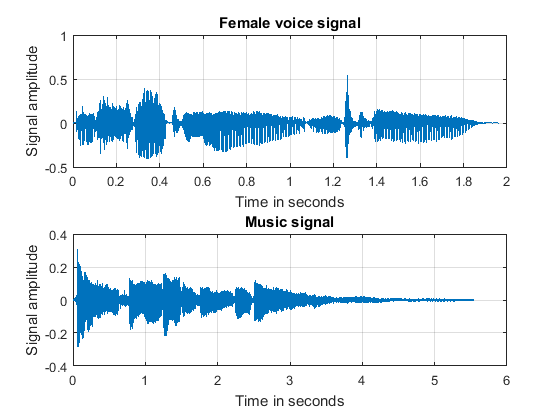
\includegraphics[width=0.77\linewidth]{./images/music_female_time.png}
		\caption{Time series of the female speech and music signal}
		\label{fig:1}	
\end{figure}

\begin{figure}[h]
\centering
\begin{minipage}{.5\textwidth}
  \centering
  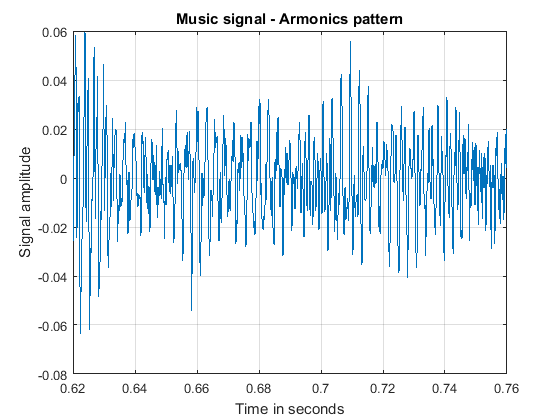
\includegraphics[width=0.95\linewidth]{./images/music_time_zoom.png}
  \captionof{figure}{Harmonic structure of the music signal}
  \label{fig:2}	
\end{minipage}%
\begin{minipage}{.5\textwidth}
  \centering
  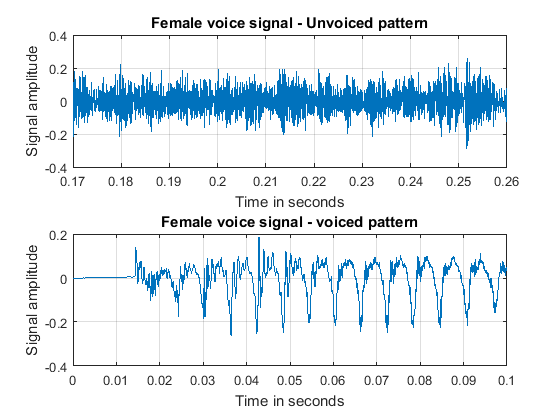
\includegraphics[width=0.95\linewidth]{./images/female_time_zoom.png}
   \captionof{figure}{Plot of unvoiced and voiced sounds of the female speech}
   \label{fig:3}	
\end{minipage}

 
\end{figure}

\newpage
\section{Speech Corpus}
In order to test the speech recognition system, a database has been recorded. The database consists of 14 different words with distinct difficulties. Multisyllabic words as \textbf{recognition} and \textbf{environment}, similar sounding words as \textbf{affect} and \textbf{effect} and short words as \textbf{I}, \textbf{am}, \textbf{in} and \textbf{is} in order to challenge the system. Other random words are added and listed in table \ref{ta:words}. Additionally, this database allows it to form some simple sentences like \textbf{I am Lars} or \textbf{Alessio is in Stockholm}, which could be tested.\\ \\\
Each word has been recorded at least 10 times, and at most 20 times, by every person listed in table \ref{ta:people}. In the end we have at least $50$ recordings for each word, making a total of at least $700$ recordings. Of the people listed in table \ref{ta:people}, only Paolo used his microphone to record the words, for all the other people each recording has been done with the same microphone(built-in mac microphone). The same settings(16 bit mono wav files with 22050 Hz) were used every time, and the software used was \textit{Audacity}. The test person is supposed to sit half a meter away from the microphone in a silent environment.
\begin{table}[ht]
\begin{tabular}{|l|l|}
\hline
\bf{Type} & \bf{Words}\\
\hline
Multisyllabic & recognition, environment\\
\hline
Similar & affect, effect\\
\hline
Short & I, am, in, is\\
\hline
Names & Alessio, Lars\\
\hline
Random & hand, chair, markov, Stockholm \\
\hline
\end{tabular}
\centering
\caption{Speech Corpus}
\label{ta:words}
\end{table}

\begin{table}[ht]
\begin{tabular}{|l|l|}
\hline
\bf{Person} & \bf{Nationality} \\
\hline
Lars & German\\
\hline
Alessio & Italian\\
\hline
Natalie & Dutch\\
\hline
Martin & Swiss\\
\hline
Paolo & Italian \\
\hline
\end{tabular}
\centering
\caption{Test person}
\label{ta:people}
\end{table}
The database contains variation in the following sense: we have people from multiple nationalities, thus different accents. Moreover, we also have a female voice and recordings done with a different microphone.
\\
\newpage
\section{Comparison: Spectrogram and Cepstrogram}
The comparison of spectrogram and cepstrogram has been performed for the combination of female speech versus music and for female speech versus male speech. The code is given by:
\begin{lstlisting}
window_length = 0.03; %in ms
num_cepstral  = 13;

[mfccs_f,spectgram_f,f_f,t_f]       = GetSpeechFeatures(y_female,...
                                fs_female,window_length,num_cepstral);
[mfccs_mu,spectgram_mu,f_mu,t_mu]   = GetSpeechFeatures(y_music,...
                                fs_music,window_length,num_cepstral);
[mfccs_ma,spectgram_ma,f_ma,t_ma]   = GetSpeechFeatures(y_male,...
                                fs_male,window_length,num_cepstral);


% mean the signal
mfccs_f = mfccs_f-repmat(mean(mfccs_f,2),1,size(mfccs_f,2));
mfccs_mu = mfccs_mu-repmat(mean(mfccs_mu,2),1,size(mfccs_mu,2));
mfccs_ma = mfccs_ma-repmat(mean(mfccs_ma,2),1,size(mfccs_ma,2));
% normalize variance to 1
norm_f   = (std(mfccs_f.')).';
mfccs_fn = mfccs_f.*repmat((1./norm_f),1,size(mfccs_f,2));
norm_m   = (std(mfccs_mu.')).';
mfccs_mn = mfccs_mu.*repmat((1./norm_m),1,size(mfccs_mu,2));
norm_ma   = (std(mfccs_ma.')).';
mfccs_man = mfccs_ma.*repmat((1./norm_ma),1,size(mfccs_ma,2));

figure(7)
subplot(2,1,1); imagesc(t_f,f_f,log10(spectgram_f)); colormap jet
xlabel('Time in seconds'); ylabel('Frequency in Hz'); title('Female voice - Spectrogram')
subplot(2,1,2); imagesc(t_mu,f_mu,log10(spectgram_mu)); colormap jet;
xlabel('Time in seconds'); ylabel('Frequency in Hz'); title('Music - Spectrogram')

figure(8)
subplot(2,1,1); imagesc(t_f,1:num_cepstral,mfccs_fn); colormap jet
xlabel('Time in seconds'); ylabel('MFCCS'); title('Female voice - Cepstrogram')
subplot(2,1,2); imagesc(t_mu,1:num_cepstral,mfccs_mn); colormap jet
xlabel('Time in seconds'); ylabel('MFCCS'); title('Music - Cepstrogram')

figure(9)
subplot(2,1,1); imagesc(t_f,f_f,log10(spectgram_f)); colormap jet
xlabel('Time in seconds'); ylabel('Frequency in Hz'); title('Female voice - Spectrogram')
subplot(2,1,2); imagesc(t_ma,f_ma,log10(spectgram_ma)); colormap jet;
xlabel('Time in seconds'); ylabel('Frequency in Hz'); title('Male voice - Spectrogram')

figure(10)
subplot(2,1,1); imagesc(t_f,1:num_cepstral,mfccs_fn); colormap jet
xlabel('Time in seconds'); ylabel('MFCCS'); title('Female voice - Cepstrogram')
subplot(2,1,2); imagesc(t_ma,1:num_cepstral,mfccs_man); colormap jet
xlabel('Time in seconds'); ylabel('MFCCS'); title('Male voice - Cepstrogram')
\end{lstlisting}

The results for the music and female speech comparison are shown in figure \ref{fig:7} and \ref{fig:8}. For a human, the spectrogram representation is easier to interpret since the all-time occurring harmonics within the music signal are very characteristic. Also, the distinction between voiced and unvoiced sounds in the speech signal are obvious. As a human, you also have kind of a physical notion for these real physical quantities that relate to certain frequencies. On the other hand, the cepstrogram is low dimensional in the sense that the amount of data has been reduced significantly, which makes it easier to handle the data within a computer. But for a human, the understanding of the pattern are much harder here. The normalised cepstrogram seems to be random on a first glance. It is hard to distinguish between voiced and unvoiced sound by looking.\\

The other comparison is shown in figure \ref{fig:9} and \ref{fig:10}. The spectrograms are similar for a human since they have kind of the same behaviour. Voiced and unvoiced parts are visible, but they are a bit blurred within the male signal. The first and third unvoiced parts are visible within the male signal, whereas these characteristic is not visible for the second unvoiced part. Also, the harmonics are more or less blurred. Hence, there are differences between the signals, but the similarities are visiblie for a human (this goes along with the fact that we know that it represents the same phrase beforehand). Due to the high amount of data and also the difference in output power and pitch between those signals, it could be hard for a computer to make this statement. The cepstrogram comparison seems random at first, but having a deeper look into it, it becomes clear that the cepstrograms share some properties, which can be handled easily by the computer. The pitch has been removed such that the harmonics don't differ anymore and also the general behaviour when comparing the coefficients are similar. For instance the third coefficient has high (red) values around $1.4$ seconds and low (blue) values around $0.4$ seconds for both male and female signal. In general it seems like the computer has an advantage here compared to a human to interpret these pictures.

\begin{figure}[h]
		\centering
		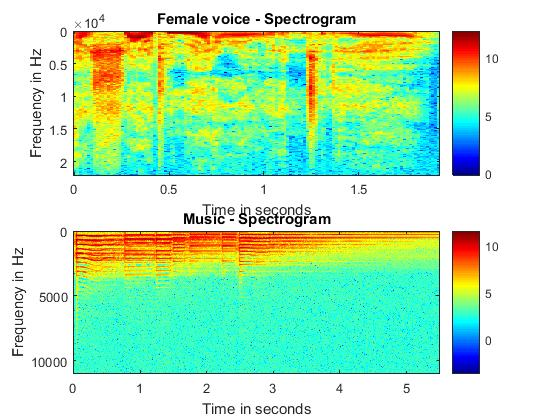
\includegraphics[width=0.77\linewidth]{./images/7.jpg}
		\caption{Spectrogram comparison: female speech vs. music signal}
		\label{fig:7}	
\end{figure}
\begin{figure}[h]
		\centering
		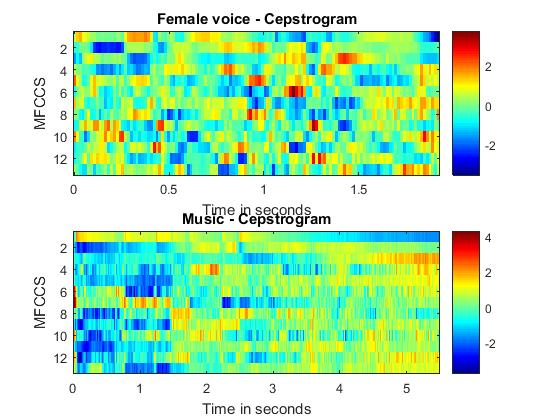
\includegraphics[width=0.75\linewidth, keepaspectratio]{./images/8.jpg}
		\caption{Cepstrogram comparison: female speech vs. music signal}
		\label{fig:8}	
\end{figure}
\pagebreak
\begin{figure}[h]
		\centering
		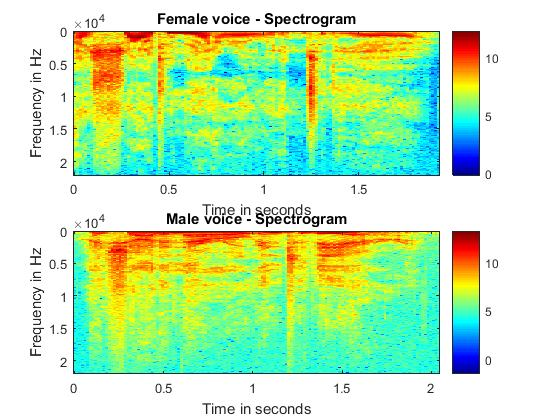
\includegraphics[width=0.75\linewidth, keepaspectratio]{./images/9.jpg}
		\caption{Spectrogram comparison: female speech vs. male speech}
		\label{fig:9}	
\end{figure}
\pagebreak
\begin{figure}[h]
		\centering
		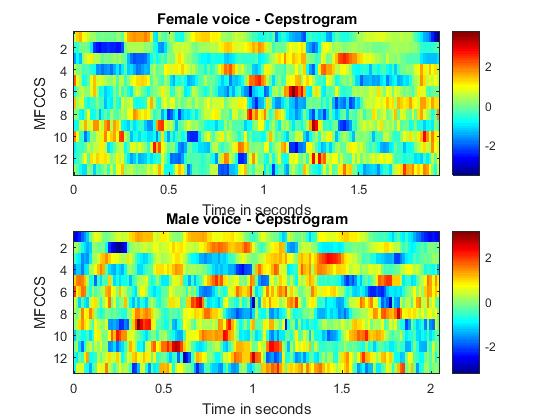
\includegraphics[width=0.75\linewidth, keepaspectratio]{./images/10.jpg}
		\caption{Cepstrogram comparison: female speech vs. male speech}
		\label{fig:10}	
\end{figure}

\end{document}